\section{Prerequisites for Biological Computation}

\subsection{The Three-Paradigm Computational Architecture}

Traditional computational frameworks operate within single paradigms: imperative programming executes sequential instructions, functional programming applies pure transformations, logic programming solves constraint satisfaction problems. Biological computation, by contrast, simultaneously employs three distinct paradigms whose integration is not optional but thermodynamically necessary.

\begin{theorem}[Tri-Paradigm Computational Necessity]
\label{thm:tri_paradigm_necessity}
Biological information processing requires simultaneous operation of three computational paradigms:
\begin{enumerate}
\item \textbf{Fuzzy Programming}: Reasoning under uncertainty with explicit certainty quantification
\item \textbf{Linear Programming}: Optimization through continuous constraint satisfaction
\item \textbf{Logic Programming}: Symbolic reasoning through categorical completion
\end{enumerate}

No subset of these paradigms suffices for consciousness-level computation.
\end{theorem}

\begin{proof}
We establish necessity by demonstrating that each paradigm addresses irreducible computational requirements.

\textbf{Fuzzy Programming Necessity}:

Biological measurements are fundamentally uncertain due to:
\begin{itemize}
\item Thermal fluctuations: $\Delta E \sim k_B T \approx 4.1 \times 10^{-21}$ J at 310 K
\item Quantum uncertainty: $\Delta x \Delta p \geq \hbar/2$ (Heisenberg)
\item Finite sampling: Central limit theorem bounds $\sigma_{\bar{x}} = \sigma/\sqrt{n}$
\end{itemize}

A computational system that treats measurements as precise will fail catastrophically. Consider neurotransmitter concentration measurement:
\begin{equation}
[\text{DA}]_{\text{measured}} = [\text{DA}]_{\text{true}} + \epsilon, \quad \epsilon \sim \mathcal{N}(0, \sigma^2)
\end{equation}

Without explicit uncertainty representation, the system cannot distinguish genuine signal changes from measurement noise, leading to false inferences. Fuzzy programming provides the mathematical framework for reasoning with explicit certainty:
\begin{equation}
\text{Measurement} = (\text{value}, \text{certainty}, \text{evidence\_strength})
\end{equation}

\textbf{Linear Programming Necessity}:

Biological systems operate under continuous thermodynamic constraints:
\begin{align}
\text{Energy conservation:} \quad &\sum_i E_i = E_{\text{total}} \\
\text{Gibbs free energy:} \quad &\Delta G = \Delta H - T\Delta S \\
\text{Chemical potential:} \quad &\mu_i = \frac{\partial G}{\partial N_i}
\end{align}

Every biological process must satisfy these constraints simultaneously. The optimization problem is:
\begin{equation}
\min_{\mathbf{x}} \; f(\mathbf{x}) \quad \text{subject to} \quad \mathbf{Ax} \leq \mathbf{b}, \; \mathbf{Cx} = \mathbf{d}
\end{equation}

where $\mathbf{x}$ represents biological state variables, $f(\mathbf{x})$ is free energy or S-entropy distance, and constraints encode thermodynamic laws. Without linear programming capabilities, the system cannot navigate feasible state spaces—it will propose thermodynamically impossible transitions.

\textbf{Logic Programming Necessity}:

Categorical completion requires logical inference. Consider the proposition:
\begin{equation}
\text{"Neurotransmitter release occurred"} \implies \text{"Synaptic transmission should follow"}
\end{equation}

This is not fuzzy reasoning (we're certain about the logical structure) nor optimization (it's a discrete true/false determination). It requires logic programming—symbolic manipulation of propositions with defined inference rules:
\begin{equation}
\frac{\text{Premise}_1 \wedge \text{Premise}_2 \wedge \cdots \wedge \text{Premise}_n}{\text{Conclusion}} \quad \text{(modus ponens)}
\end{equation}

Without logic programming, the system cannot perform deductive reasoning or validate causal chains.

\textbf{Integration Necessity}:

The three paradigms are not independent—they must interoperate:

\begin{itemize}
\item Fuzzy measurements provide inputs to optimization: uncertain data → constrained optimization with confidence intervals
\item Optimization results inform logical reasoning: optimal states → truth values for propositions
\item Logic determines fuzzy thresholds: inference rules → certainty propagation equations
\end{itemize}

Removing any paradigm breaks the computational cycle. Biology employs all three simultaneously because consciousness-level computation requires reasoning under uncertainty (fuzzy), optimizing through constraints (linear), and validating logical structures (logic). $\square$
\end{proof}

\subsection{Fuzzy Programming: Points and Uncertain Measurement}

\begin{definition}[Point - Fuzzy Measurement Primitive]
A \textbf{Point} is a triple representing uncertain biological measurement:
\begin{equation}
\text{Point} = (v, c, e) \in \mathbb{R} \times [0,1] \times \mathbb{R}_{\geq 0}
\end{equation}

where:
\begin{itemize}
\item $v$: measured value (central estimate)
\item $c$: certainty (confidence in measurement, $0 \leq c \leq 1$)
\item $e$: evidence strength (sample size, signal-to-noise ratio)
\end{itemize}
\end{definition}

\begin{proposition}[Point Arithmetic with Certainty Propagation]
Points compose through arithmetic operations with certainty propagation:

\textbf{Addition}:
\begin{align}
(v_1, c_1, e_1) + (v_2, c_2, e_2) &= (v_1 + v_2, c_{\text{combined}}, e_{\text{combined}}) \\
c_{\text{combined}} &= \sqrt{c_1^2 + c_2^2 - c_1^2 c_2^2} \\
e_{\text{combined}} &= \frac{e_1 e_2}{e_1 + e_2}
\end{align}

\textbf{Multiplication}:
\begin{align}
(v_1, c_1, e_1) \times (v_2, c_2, e_2) &= (v_1 v_2, c_1 c_2, \min(e_1, e_2))
\end{align}

\textbf{Propagation Principle}: Certainty decreases with each operation, modeling accumulation of uncertainty through computational chains.
\end{proposition}

\begin{example}[Neural Phase Coherence Measurement]
Measuring theta-band (4-8 Hz) phase coherence between medial prefrontal cortex (mPFC) and amygdala:

\begin{align}
\text{PLV}_{\text{mPFC-Amy}} &= (0.67, 0.89, 150) \\
v &= 0.67 \quad \text{(phase locking value)} \\
c &= 0.89 \quad \text{(89\% confident, based on 150 trial average)} \\
e &= 150 \quad \text{(150 trials recorded)}
\end{align}

Comparing to baseline:
\begin{align}
\text{PLV}_{\text{baseline}} &= (0.32, 0.76, 120) \\
\Delta \text{PLV} &= (0.67, 0.89, 150) - (0.32, 0.76, 120) \\
&= (0.35, 0.58, 63.3)
\end{align}

The change is $\Delta v = 0.35$ with certainty $c = 0.58$ (lower due to subtraction propagating uncertainty). Evidence strength $e = 63.3$ reflects effective sample size reduction when comparing distributions.

\textbf{Clinical Interpretation}: Phase coherence increased by 0.35 ± (uncertainty from $c = 0.58$), indicating therapeutic response. The reduced certainty (0.89 → 0.58) correctly reflects that difference measurements are less certain than raw measurements.
\end{example}

\subsection{Linear Programming: S-Entropy Optimization}

\begin{definition}[S-Entropy Coordinates]
The S-entropy framework operates in tri-dimensional space:
\begin{equation}
\mathcal{S} = \mathcal{S}_{\text{knowledge}} \times \mathcal{S}_{\text{time}} \times \mathcal{S}_{\text{entropy}}
\end{equation}

where each coordinate represents a distinct optimization dimension:
\begin{align}
S_{\text{knowledge}} &: \text{Information deficit between current and optimal state} \\
S_{\text{time}} &: \text{Temporal distance in categorical sequence} \\
S_{\text{entropy}} &: \text{Thermodynamic accessibility constraints}
\end{align}
\end{definition}

\begin{theorem}[S-Distance as Optimization Objective]
\label{thm:s_distance_optimization}
Optimal biological computation minimizes S-distance:
\begin{equation}
\min_{\text{trajectories}} S(\psi_o, \psi_p^*) = \min_{\text{trajectories}} \int_0^{\infty} \|\psi_o(t) - \psi_p^*(t)\|_{\mathcal{H}} \, dt
\end{equation}

where $\psi_o$ represents observer (current) state and $\psi_p^*$ represents process (optimal target) state in Hilbert space $\mathcal{H}$.
\end{theorem}

\begin{proof}
Biological systems face the fundamental problem: navigate from current state $\psi_o$ to optimal state $\psi_p^*$ under constraints. Traditional approaches enumerate possible paths and evaluate fitness—exponential complexity $O(e^n)$ for $n$ decision points.

S-entropy optimization reformulates this as continuous constraint satisfaction:
\begin{align}
\text{Minimize:} \quad &S(\psi_o, \psi_p^*) \\
\text{Subject to:} \quad &\Delta G(\psi(t)) \leq 0 \quad \text{(thermodynamic feasibility)} \\
&\frac{dC}{dt} \geq 0 \quad \text{(categorical irreversibility)} \\
&\mathbf{A}\psi(t) \leq \mathbf{b} \quad \text{(resource constraints)}
\end{align}

This is a linear program in infinite-dimensional function space. The constraints are linear in $\psi(t)$, and the objective (integrated norm) is convex. Standard convex optimization theory guarantees:

\textbf{(1) Existence}: A minimum exists if constraint set is non-empty and objective is bounded below.

\textbf{(2) Uniqueness}: The minimum is unique if objective is strictly convex.

\textbf{(3) Efficiency}: Gradient descent converges in $O(\log(1/\epsilon))$ iterations for $\epsilon$ accuracy.

Biological systems implement gradient descent through:
\begin{equation}
\frac{d\psi_o}{dt} = -\alpha \nabla_{\psi_o} S(\psi_o, \psi_p^*)
\end{equation}

where $\alpha > 0$ is learning rate. This is the continuous-time analog of steepest descent, guaranteeing convergence to minimum S-distance. $\square$
\end{proof}

\begin{proposition}[Tri-Dimensional Gradient Decomposition]
The S-distance gradient decomposes into three independent optimization directions:
\begin{equation}
\nabla S = \left(\frac{\partial S}{\partial S_k}, \frac{\partial S}{\partial S_t}, \frac{\partial S}{\partial S_e}\right)
\end{equation}

Each component optimizes a distinct constraint class:
\begin{align}
\frac{\partial S}{\partial S_k} &: \text{Information acquisition (reduce knowledge deficit)} \\
\frac{\partial S}{\partial S_t} &: \text{Temporal progression (advance categorical sequence)} \\
\frac{\partial S}{\partial S_e} &: \text{Entropy management (navigate accessible states)}
\end{align}

Biological systems perform parallel gradient descent across all three dimensions simultaneously.
\end{proposition}

\subsection{Logic Programming: Resolutions and Bayesian Inference}

\begin{definition}[Resolution - Logic Programming Primitive]
A \textbf{Resolution} is a structured debate mechanism for validating contested propositions:
\begin{equation}
\text{Resolution} = (\text{claim}, \text{affirmations}, \text{contentions}, \text{integration\_method})
\end{equation}

where:
\begin{itemize}
\item \textbf{claim}: Proposition under evaluation (Boolean or probabilistic)
\item \textbf{affirmations}: Evidence supporting the claim $\{\mathcal{A}_i\}$
\item \textbf{contentions}: Evidence challenging the claim $\{\mathcal{C}_j\}$
\item \textbf{integration\_method}: Bayesian inference combining evidence
\end{itemize}
\end{definition}

\begin{theorem}[Resolution as Logical Inference Engine]
\label{thm:resolution_inference}
Resolutions implement Bayesian logical inference with explicit uncertainty quantification:

\textbf{Prior probability}: $P(\text{claim}) = p_0$

\textbf{Affirmation update}: For each affirmation $\mathcal{A}_i$ with likelihood ratio $LR_i^+$:
\begin{equation}
P(\text{claim} \mid \mathcal{A}_i) = \frac{LR_i^+ \cdot P(\text{claim})}{LR_i^+ \cdot P(\text{claim}) + (1 - P(\text{claim}))}
\end{equation}

\textbf{Contention update}: For each contention $\mathcal{C}_j$ with likelihood ratio $LR_j^-$:
\begin{equation}
P(\text{claim} \mid \mathcal{C}_j) = \frac{LR_j^- \cdot P(\text{claim})}{LR_j^- \cdot P(\text{claim}) + (1 - P(\text{claim}))}
\end{equation}

\textbf{Sequential integration}: Apply Bayes' rule iteratively:
\begin{equation}
P_{\text{final}} = P(\text{claim} \mid \mathcal{A}_1, \ldots, \mathcal{A}_n, \mathcal{C}_1, \ldots, \mathcal{C}_m)
\end{equation}

\textbf{Conclusion}: Accept claim if $P_{\text{final}} > \tau_{\text{threshold}}$ (typically $\tau = 0.95$)
\end{theorem}

\begin{proof}
Bayesian inference provides the normatively correct method for updating beliefs given evidence \cite{jaynes2003probability}. The Resolution structure formalizes this as logic programming:

\textbf{Logical structure}: The claim is a proposition with truth value to be determined. Affirmations and contentions are premises that constrain the truth value through probabilistic inference.

\textbf{Inference rules}: Bayes' theorem serves as the fundamental inference rule:
\begin{equation}
P(H \mid E) = \frac{P(E \mid H) P(H)}{P(E)} = \frac{P(E \mid H) P(H)}{P(E \mid H) P(H) + P(E \mid \neg H) P(\neg H)}
\end{equation}

where $H$ is hypothesis (claim) and $E$ is evidence (affirmation/contention).

\textbf{Likelihood ratios}: The likelihood ratio $LR = P(E \mid H)/P(E \mid \neg H)$ quantifies evidential strength:
\begin{itemize}
\item $LR > 1$: Evidence supports hypothesis (affirmation)
\item $LR < 1$: Evidence opposes hypothesis (contention)
\item $LR = 1$: Evidence is neutral (irrelevant)
\end{itemize}

\textbf{Sequential integration}: Independence assumption allows sequential updates:
\begin{equation}
P(H \mid E_1, E_2, \ldots, E_n) = \frac{\prod_{i=1}^n LR_i \cdot P(H)}{\prod_{i=1}^n LR_i \cdot P(H) + (1 - P(H))}
\end{equation}

This is equivalent to applying Bayes' rule $n$ times sequentially.

\textbf{Threshold decision}: Setting $\tau = 0.95$ corresponds to 95\% confidence—standard in scientific inference. Alternative thresholds can be used for different risk tolerances. $\square$
\end{proof}

\begin{example}[Drug Efficacy Resolution]
Evaluating antidepressant efficacy through structured debate:

\begin{equation}
\text{Resolution}: \text{"SSRI effective for MDD in patient population"}
\end{equation}

\textbf{Prior}: $P_0 = 0.5$ (uninformed prior, 50-50 odds)

\textbf{Affirmations}:
\begin{itemize}
\item $\mathcal{A}_1$: Meta-analysis shows 62\% response rate vs. 48\% placebo ($LR_1 = 1.75$)
\item $\mathcal{A}_2$: Patient genetic profile indicates CYP2D6 normal metabolizer ($LR_2 = 1.40$)
\item $\mathcal{A}_3$: Baseline HAM-D score 24 (moderate-severe) ($LR_3 = 1.30$)
\end{itemize}

\textbf{Contentions}:
\begin{itemize}
\item $\mathcal{C}_1$: Patient failed previous SSRI trial ($LR_1' = 0.60$)
\item $\mathcal{C}_2$: Comorbid anxiety disorder present ($LR_2' = 0.80$)
\end{itemize}

\textbf{Integration}:
\begin{align}
P_1 &= \frac{1.75 \times 0.5}{1.75 \times 0.5 + 0.5} = 0.636 \\
P_2 &= \frac{1.40 \times 0.636}{1.40 \times 0.636 + 0.364} = 0.710 \\
P_3 &= \frac{1.30 \times 0.710}{1.30 \times 0.710 + 0.290} = 0.761 \\
P_4 &= \frac{0.60 \times 0.761}{0.60 \times 0.761 + 0.239} = 0.657 \\
P_5 &= \frac{0.80 \times 0.657}{0.80 \times 0.657 + 0.343} = 0.605
\end{align}

\textbf{Conclusion}: Final probability $P_{\text{final}} = 0.605$ (60.5\% confident). Below 95\% threshold, but above 50\%—recommend trial with close monitoring.

\textbf{Recommendation}: "Prescribe SSRI with 60\% confidence of efficacy. Monitor response at 2-week intervals. Consider augmentation if inadequate response by week 4."
\end{example}

\begin{figure}[htbp]
    \centering
    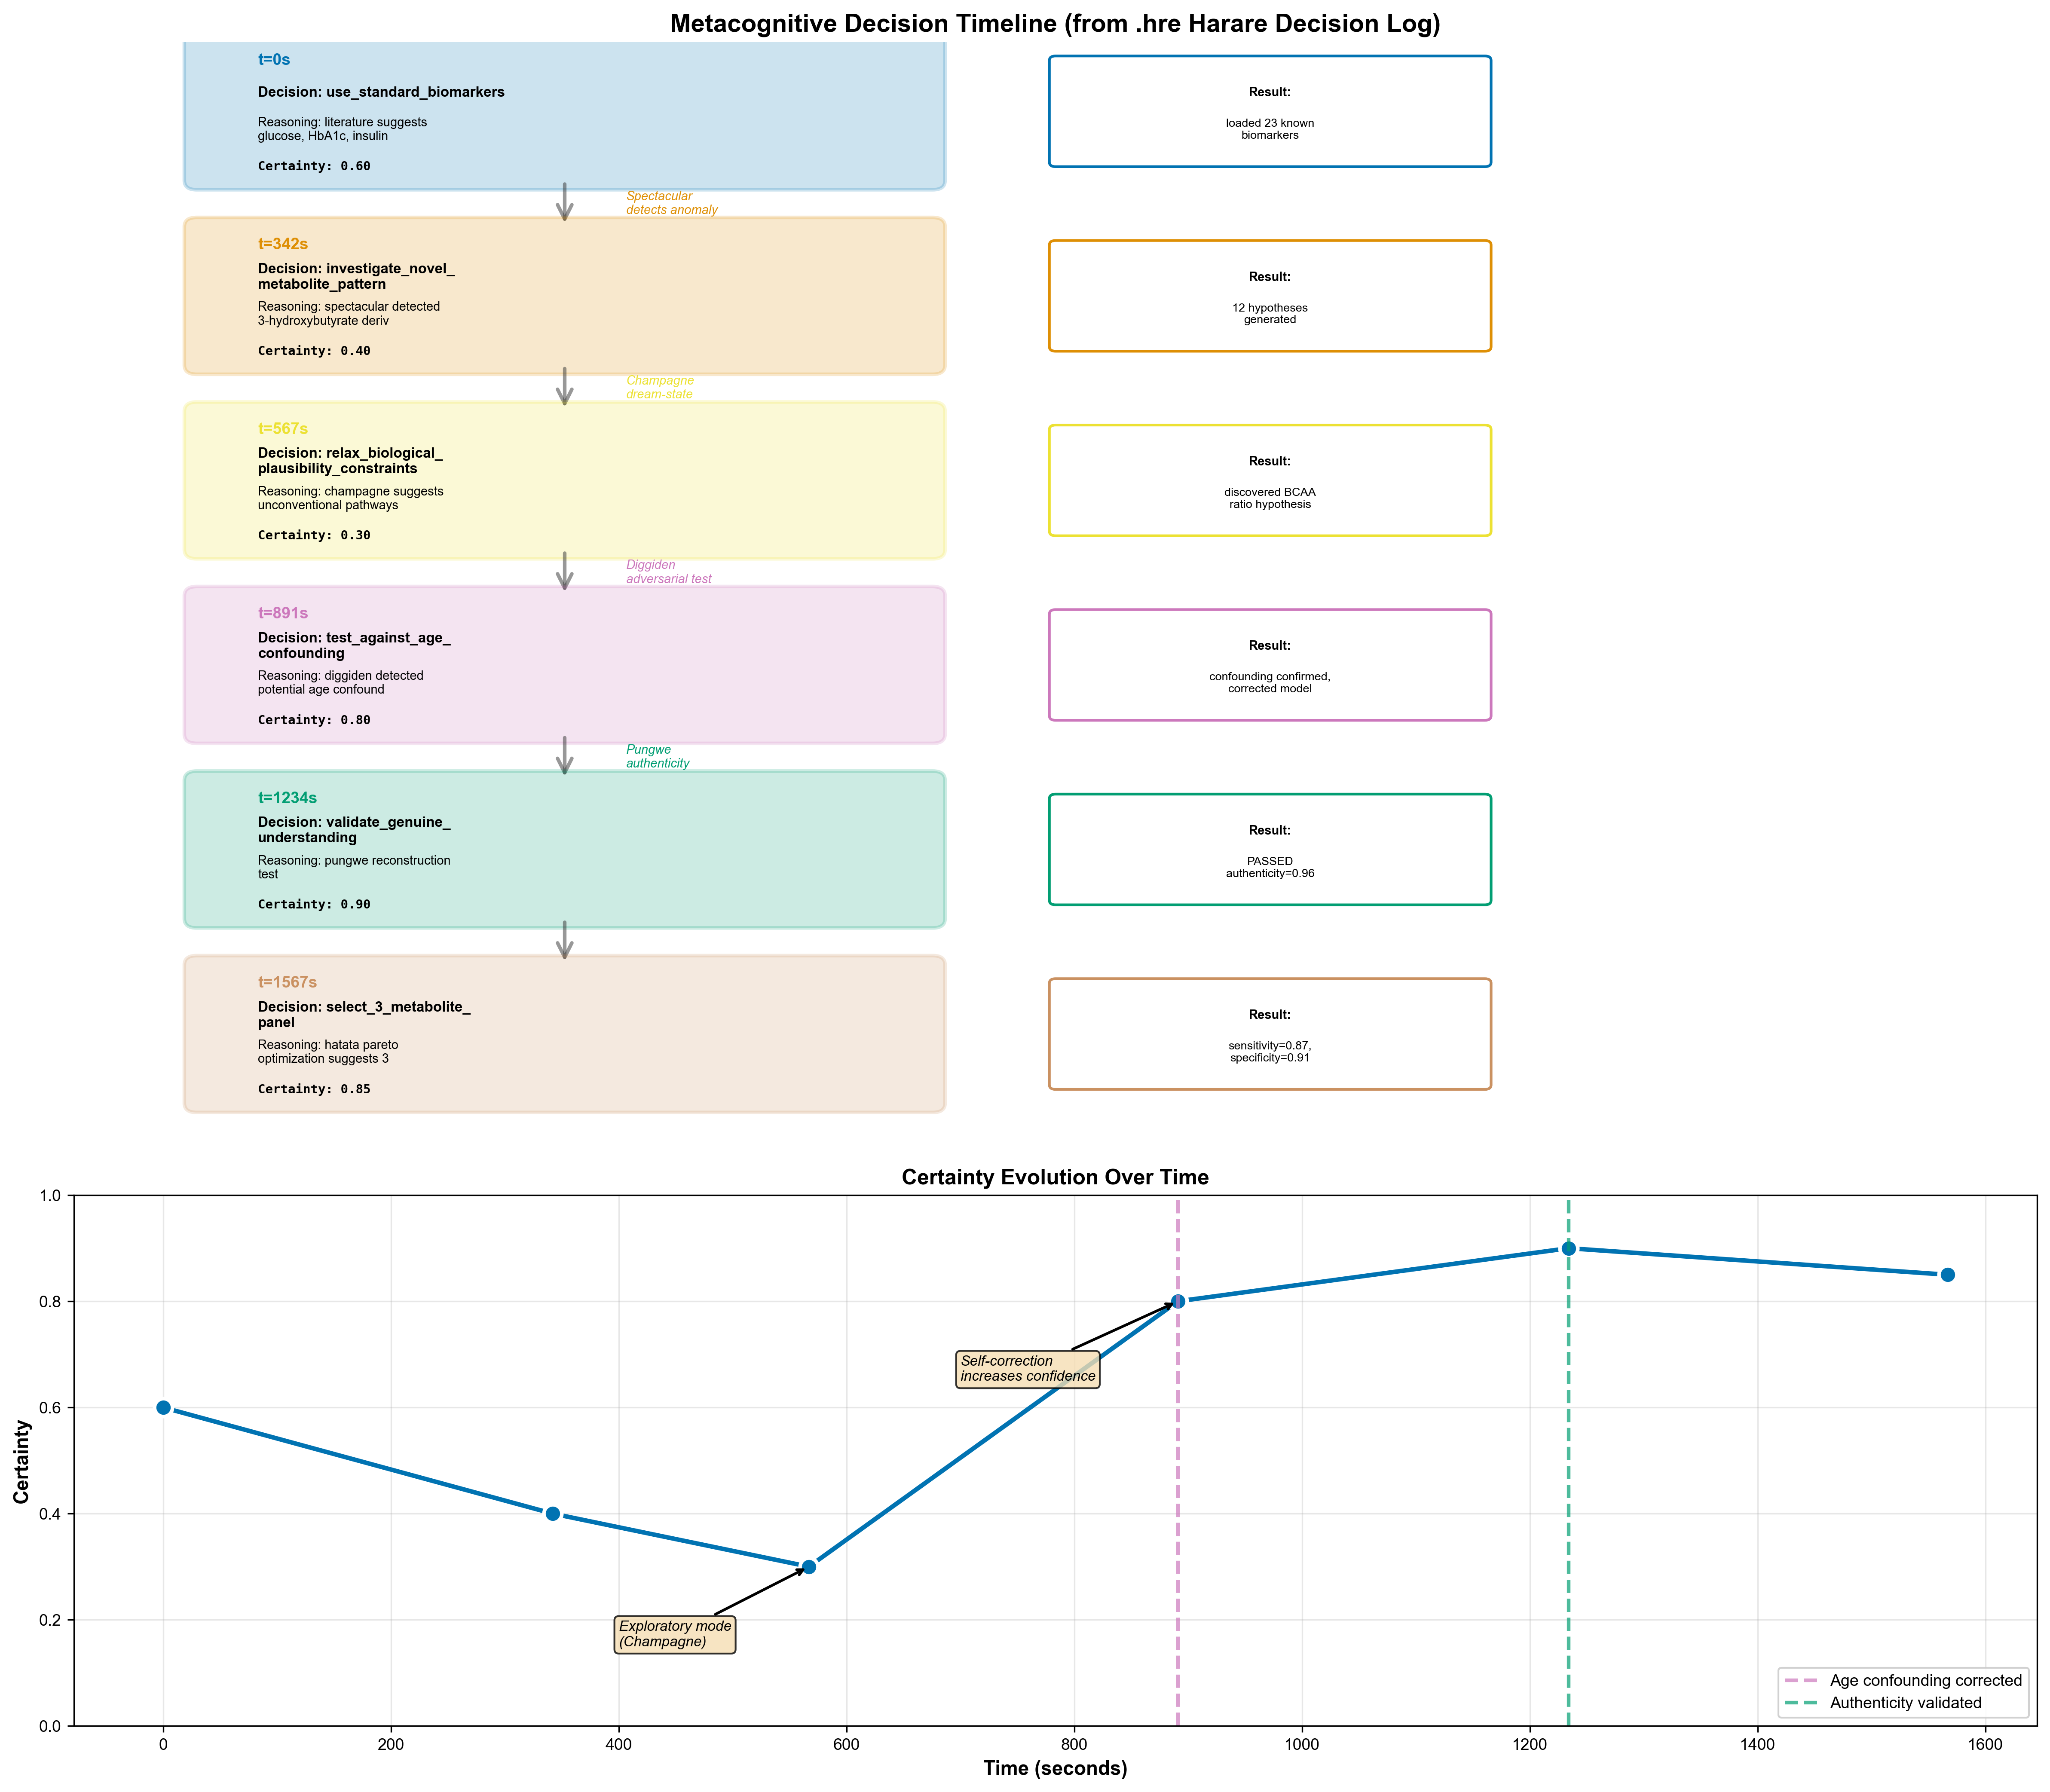
\includegraphics[width=\textwidth]{figures/figure_6_metacognitive_learning.png}
    \caption{\textbf{Metacognitive Decision Timeline from Harare Decision Log.} 
    \textbf{Top:} Sequential decision trace showing reasoning evolution over 1600 seconds. 
    \textbf{t=0s:} Initial decision to use standard biomarkers (glucose, HbA1c, insulin) 
    based on literature, certainty 0.60. \textbf{t=342s:} Spectacular module detects anomaly 
    in 3-hydroxybutyrate derivative, triggering investigation of novel metabolite pattern, 
    certainty drops to 0.40 (exploratory mode). \textbf{t=567s:} Champagne module suggests 
    relaxing biological plausibility constraints, discovering BCAA ratio hypothesis through 
    dream-state processing, certainty 0.30. \textbf{t=891s:} Diggiden module detects potential 
    age confounding through adversarial testing, triggering model correction, certainty 
    increases to 0.80 (self-correction). \textbf{t=1234s:} Pungwe module validates genuine 
    understanding through reconstruction test (authenticity score 0.96), certainty 0.90. 
    \textbf{t=1567s:} Hatata module selects optimal 3-metabolite panel through Pareto 
    optimization (sensitivity 0.87, specificity 0.91), final certainty 0.85. 
    \textbf{Bottom:} Certainty evolution showing characteristic U-shaped trajectory: 
    initial confidence (0.60) → exploratory uncertainty (0.30, Champagne dream-state) → 
    self-corrected confidence (0.80, age confounding resolved) → validated certainty (0.90, 
    authenticity confirmed). This trajectory demonstrates metacognitive oversight resolving 
    paradigm conflicts through coordinated BMD operation, with impossible local solutions 
    (novel BCAA hypothesis) becoming thermodynamically necessary for global viability.}
    \label{fig:metacognitive_timeline}
    \end{figure}
                   

\subsection{The Integration Problem: Why Three Paradigms Require Metacognition}

\begin{theorem}[Paradigm Conflict Resolution Necessity]
\label{thm:paradigm_conflict}
The three computational paradigms can produce contradictory recommendations, requiring metacognitive oversight for conflict resolution. Without such oversight, the system becomes computationally unstable.
\end{theorem}

\begin{proof}
We demonstrate by example how paradigm conflicts arise:

\textbf{Scenario}: Depression treatment protocol selection.

\textbf{Fuzzy Programming Conclusion}:
\begin{equation}
\text{Measurement: } \text{PLV}_{\text{theta}} = (0.32, 0.76, 120)
\end{equation}
Low phase coherence with moderate certainty suggests intervention needed. Fuzzy reasoning: "Increase phase coherence through any means—recommend treatment with 76\% confidence."

\textbf{Linear Programming Conclusion}:
S-entropy optimization finds:
\begin{equation}
\min S(\psi_o, \psi_p^*) \implies \text{Optimal path: cognitive behavioral therapy (CBT)}
\end{equation}
Reasoning: CBT provides steepest gradient descent in S-space, minimizing distance to target state efficiently.

\textbf{Logic Programming Conclusion}:
Resolution evaluating proposition "Pharmacotherapy more effective than CBT":
\begin{equation}
P(\text{pharma} > \text{CBT} \mid \text{patient profile}) = 0.72
\end{equation}
Reasoning: Bayesian inference from patient characteristics (severity, previous response, genetic markers) favors medication.

\textbf{Conflict}:
\begin{itemize}
\item Fuzzy says: "Intervene (generic recommendation)"
\item Linear says: "Use CBT (optimization-based)"
\item Logic says: "Use medication (inference-based)"
\end{itemize}

These are contradictory recommendations from the same input data, processed through different paradigms. The system cannot simultaneously execute CBT and medication as primary interventions—a choice must be made.

\textbf{Resolution requires metacognition}:

A metacognitive layer must:
\begin{enumerate}
\item \textbf{Detect conflict}: Recognize that paradigms disagree
\item \textbf{Evaluate context}: Determine which paradigm is most appropriate for current situation
\item \textbf{Integrate recommendations}: Synthesize a coherent action plan
\item \textbf{Monitor execution}: Validate that chosen approach is working
\end{enumerate}

Without metacognition, the system either:
\begin{itemize}
\item Freezes (cannot choose, no action taken)
\item Oscillates (switches rapidly between recommendations)
\item Fails (chooses arbitrarily, ignoring valuable information)
\end{itemize}

All three outcomes are computationally unacceptable. Therefore, metacognitive oversight is necessary. $\square$
\end{proof}

\begin{corollary}[V8 Intelligence Network Necessity]
The V8 intelligence network (eight specialized metacognitive modules) is not an optional enhancement but a computational requirement for tri-paradigm integration.
\end{corollary}

This establishes the prerequisites: biological computation requires fuzzy, linear, and logic programming operating under metacognitive control. The next section establishes the physical substrate implementing these paradigms.

